% Klein coordinates: the diagonals are genuine h-lines; angles are not conformal.
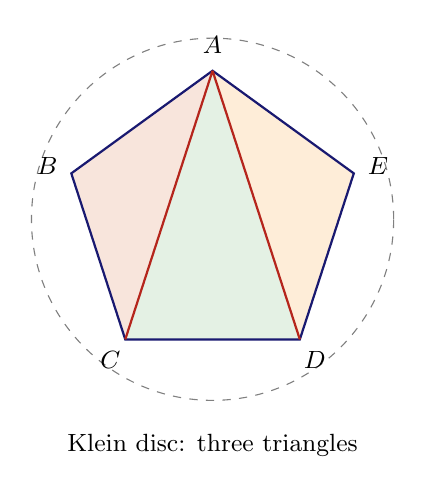
\begin{tikzpicture}[scale=2.3,font=\small]
\draw[gray,dashed] (0,0) circle (1);
\foreach \name/\ang in {A/90,B/162,C/234,D/306,E/18}{
  \coordinate (\name) at (\ang:.82);
  \node at (\ang:.96) {$\name$};
}
\fill[BrickRed!9] (A)--(B)--(C)--cycle;
\fill[ForestGreen!12] (A)--(C)--(D)--cycle;
\fill[BurntOrange!13] (A)--(D)--(E)--cycle;
\draw[MidnightBlue,thick] (A)--(B)--(C)--(D)--(E)--cycle;
\draw[BrickRed,thick] (A)--(C) (A)--(D);
\node at (0,-1.25) {Klein disc: three triangles};
\end{tikzpicture}
